\documentclass{article}
\usepackage{amsmath}
\usepackage{enumitem}
\usepackage{graphicx}
\usepackage{listings}
\usepackage{color} %red, green, blue, yellow, cyan, magenta, black, white

\title{Assignment1}
\author{Jakub Slowinski}
\begin{document}
\begin{itemize}
\item Q2.31

\definecolor{mygreen}{RGB}{28,172,0} % color values Red, Green, Blue
\definecolor{mylilas}{RGB}{170,55,241}
\lstset{language=Matlab,%
    %basicstyle=\color{red},
    breaklines=true,%
    morekeywords={matlab2tikz},
    keywordstyle=\color{blue},%
    morekeywords=[2]{1}, keywordstyle=[2]{\color{black}},
    identifierstyle=\color{black},%
    stringstyle=\color{mylilas},
    commentstyle=\color{mygreen},%
    showstringspaces=false,%without this there will be a symbol in the places where there is a space
    numbers=left,%
    numberstyle={\tiny \color{black}},% size of the numbers
    numbersep=9pt, % this defines how far the numbers are from the text
    emph=[1]{for,end,break},emphstyle=[1]\color{red}, %some words to emphasise
    %emph=[2]{word1,word2}, emphstyle=[2]{style},    
}


\section*{Matlab Code}

\lstinputlisting{Determinant.m}
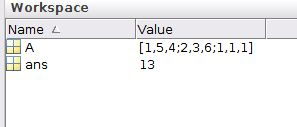
\includegraphics{deta1.png}
\\
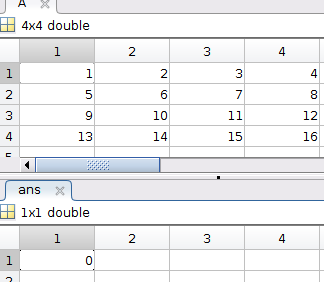
\includegraphics{detbi.png}
\\

\item Q3.2
  \\ root of f(x) = x - $2e^{-x}$
  \begin{enumerate}[label=(\alph*)]
  \item Bisection method
  \[ a=0, b=1\]
  \[f(0)=0-2e^0=-2\]
  \[f(1)=1-2e^{-1}=0.2642 \]
  \\First iteration:
  \[ x_1 = \frac{a+b}{2} = \frac{0+1}{2} = 0.5 \]
  \[f(x_1)=0.5 - 2e^{-0.5}=-0.7 \]
  \\ as this is a negative number and you need a negative value and positive value between a and b; a now equals $c_1$ 
  \\Second iteration:
  \[ a=0.5, b=1\]
  \[ x_2 = \frac{0.5+1}{2}=0.75 \]
  \[f(x_2)=0.75 - 2e^{-0.75}=-0.1947 \]
  \\ as this is a negative number, it replaces the previous negative number, a
  \\Third iteration:
  \[ a=0.75, b=1\]
  \[ x_3 = \frac{0.75+1}{2}=0.875 \]
  \[f(x_3)=0.875 - 2e^{-0.875}=0.04 \]
  \\ as this is a positive number, this is the new b
  \\Final iteration:
  \[ a=0.75, b=0.875\]
  \[ x_4 = \frac{0.75+0.875}{2}=0.8125 \]
  
  \item Secant method
  \[x_1 = 0, x_2=1 \]
  \[f(x_1)= 0-2e^0=-2 \]
  \[f(x_2)= 1-2e^{-1}=0.2642\]
  \\First iteration
  \[x_3 = x_2 - f(x_2) * \frac{x_2-x_1}{f(x_2)-f(x_1)}\]
  \[ x_3= 1-0.2642*\frac{1-0}{0.2642+2} =0.8516 \]
  \[f(x_3)= 0.8833-2e^{-0.8833}=0.0565 \]
  \\Second iteration
  \[x_4 = x_3 - f(x_3) * \frac{x_3-x_2}{f(x_3)-f(x_2)}\]
  \[x_4=0.8833-0.0565*\frac{0.8833-1}{0.0565-0.2642} =0.8516\]  
  \[f(x_4)= 0.8516-2e^{-0.8516}=-0.0019 \]
  
  Third iteration
  \[x_5 = x_4 - f(x_4) * \frac{x_4-x_3}{f(x_4)-f(x_3)}\]
  \[x_5=0.8516+0.0019*\frac{0.8516-0.8833}{-0.019-0.0565} =0.8529\]  
  \[f(x_5)= 0.8529-2e^{-0.8529}=0.00054 \]
  
  Final iteration
  \[x_6 = x_5 - f(x_5) * \frac{x_5-x_4}{f(x_5)-f(x_4)}\]
  \[x_6=0.8529-0.00054*\frac{0.8529-0.8516}{0.00054+0.0019} =0.85261\]  
    
  \item Newton's method
  \[ f(x) = x-2e^{-x}, x_1=1 \]
  \[ f'(x)=2e^{-x}+1\]
  \[ f(x_1)= 1-2e^{-1}=0.2642\]
  \[ f'(x_1)=2e^{-1}+1=1.7358\]
  
  First iteration
  \[ x_2=x_1 - \frac{f(x_1)}{f'(x_1)}\]
  \[ x_2=1 - \frac{0.2642}{1.7358}=0.8478\]
  \[ f(x_2)= 0.8478-2e^{-0.8478}=-0.0089\]
  \[ f'(x_2)=2e^{-0.8478}+1=1.8567\]
  
  Second iteration
  \[ x_3=x_2 - \frac{f(x_2)}{f'(x_2)}\]
  \[ x_3=0.8478 - \frac{-0.0089}{1.8467}=0.8526\]
  \[ f(x_2)= 0.8526-2e^{-0.8526}=-0.0001\]
  \[ f'(x_2)=2e^{-0.8526}+1=1.8526\]
  
  Third iteration
  \[ x_4=x_3 - \frac{f(x_3)}{f'(x_3)}\]
  \[ x_4=0.8526 - \frac{-0.00001}{1.8526}=0.8526\]
  \[ f(x_4)= 0.8526-2e^{-0.8526}=-0.0001\]
  \[ f'(x_4)=2e^{0.8526}+1=1.8567\]
  
  Final iteration
  \[ x_5=0.8526 - \frac{-0.00001}{1.8526}=0.8256\]
  \end{enumerate}
\item Q4.24
\\
\section*{Matlab Code}
\lstinputlisting{Inverse.m}
\begin{figure}[htbp]
\hspace*{-2cm}
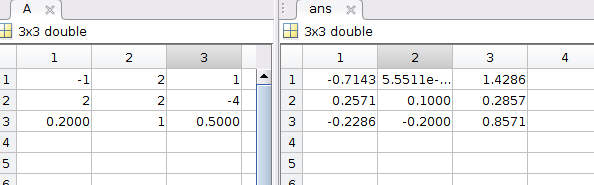
\includegraphics[scale=0.65]{3i.png}
\\
\hspace*{-2cm}
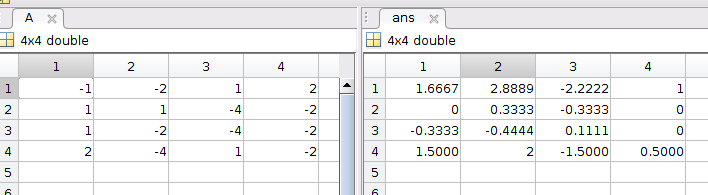
\includegraphics[scale=0.65]{3ii.png}
\end{figure}


\end{itemize}
\end{document}